\section{Principles}

\begin{frame}
\frametitle{Set your goals}
\begin{columns}
    \column{0.75\textwidth}
    \begin{itemize}
	\item Reducing boot time implies measuring boot time!
	\item You will have to choose reference events at which you
       	      start and stop counting time.
	\item What you choose will depend on the goal you want to
              achieve. Here are typical cases:
	\begin{itemize}
		\item Showing a splash screen or an animation, playing a sound to
	              indicate the board is booting
		\item Starting a listening service to handle a particular
	              message
	        \item Being fully functional as fast as possible
	\end{itemize}
    \end{itemize}
    \column{0.25\textwidth}
    % From http://openclipart.org/detail/46075/stop-watch-by-klaasvangend
    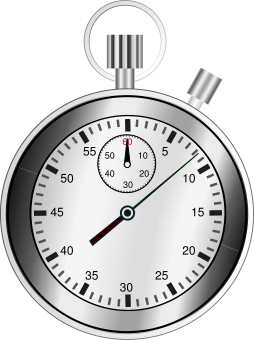
\includegraphics[width=\textwidth]{slides/boottime-principles/stop-watch.pdf}
  \end{columns}
\end{frame}

\begin{frame}
\frametitle{Boot time reduction methodology}
\begin{center}
    \includegraphics[width=\textwidth]{slides/boottime-principles/methodology.pdf}
\end{center}
\end{frame}

\begin{frame}
\frametitle{Boot time components}
Generic boot sequence
\begin{center}
    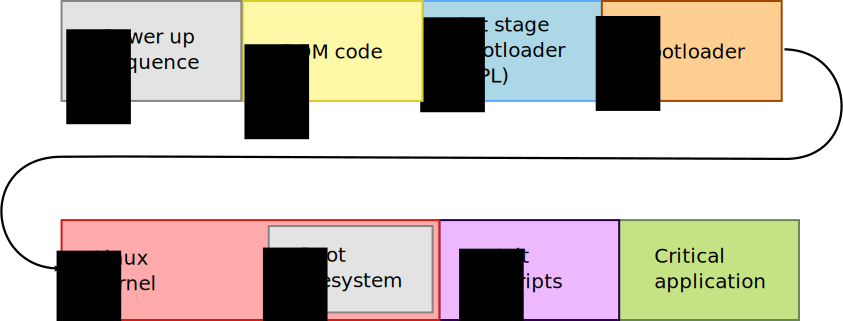
\includegraphics[width=\textwidth]{slides/boottime-principles/generic-boot-sequence.pdf}
\end{center}
Example: typical boot sequence on Atmel AT91
\begin{center}
    \includegraphics[width=\textwidth]{slides/boottime-principles/at91-boot-sequence.pdf}
\end{center}
We are focusing on reducing {\em cold} boot time, from power on to the
critical application.
\end{frame}

\begin{frame}
\frametitle{Main advice: worst things first!}
{\em Premature optimization is the root of all evil.\\
Donald Knuth}     
\begin{itemize}
\item Taking the time to measure time carefully is important.
\item Find the worst consumers of time and address them first.
\item You can waste a lot of time if you start optimizing
      minor spots first.
\end{itemize}
\end{frame}


\begin{frame}
\frametitle{Key ideas}
Some ideas to keep in mind while trying to reduce the boot time:
\begin{itemize}
\item The fastest code is code that is not executed
\item A big part of booting is actually loading code and data from the
        storage to RAM. Reading less means booting faster. I/O are
        expensive !
\item The root filesystem may take longer to mount if it is bigger.
\item So, even code that is not executed can make your boot time
        longer.
\item Also, try to benchmark different types of storage. It has
        happened that booting from SD card was actually faster than
        booting from NAND.
\item It may be worth playing with gcc options like \code{-Os} to
generate
        smaller code but then, you will have to measure the performance.
        It may or may not be worse.
\end{itemize}
\end{frame}

\setuplabframe
{Getting started}
{
\begin{itemize}
\item Learn how to interact with the board
\item Learn how to flash it 
\end{itemize}
}

